\chapter{Sprint1: Configuration de l'architecture cloud AWS.}
\newpage
\textbf{\huge Introduction} \\[1cm]
\textsf{\fontfamily{qtm}\selectfont\scalefont{1.3}
Après avoir déduit le besoin de du projet et identifie les acteurs nous présentent le premier sprint, nous commençons par l'objectif de sprint puis l'architecture globale ensuite nous détaillons le diagramme d'utilisation et séquence détaille, Finalement, nous allons exposer la partie réalisation}


\section{\LARGE Objectif du Sprint}
\textsf{\fontfamily{qtm}\selectfont\scalefont{1.3}Ce sprint a pour but de configurer l'architecture cloud qui en va l'utiliser dans notre projet, la solution cloud choisit et l'hybride cloud nous allons configurer une VPC puis connectée à notre data center a travers un VPN finalement nous allons configurer un cluster EKS et établir une connexion entre une machine locale et le cluster.}


\section{\LARGE Architecture Global}
\textsf{\fontfamily{qtm}\selectfont\scalefont{1.3}
Dans cette partie en va proposer l'architecture globale utilisée pour la configuration de l'infrastructure cloud. }

\begin{figure}[H]
\begin{center}
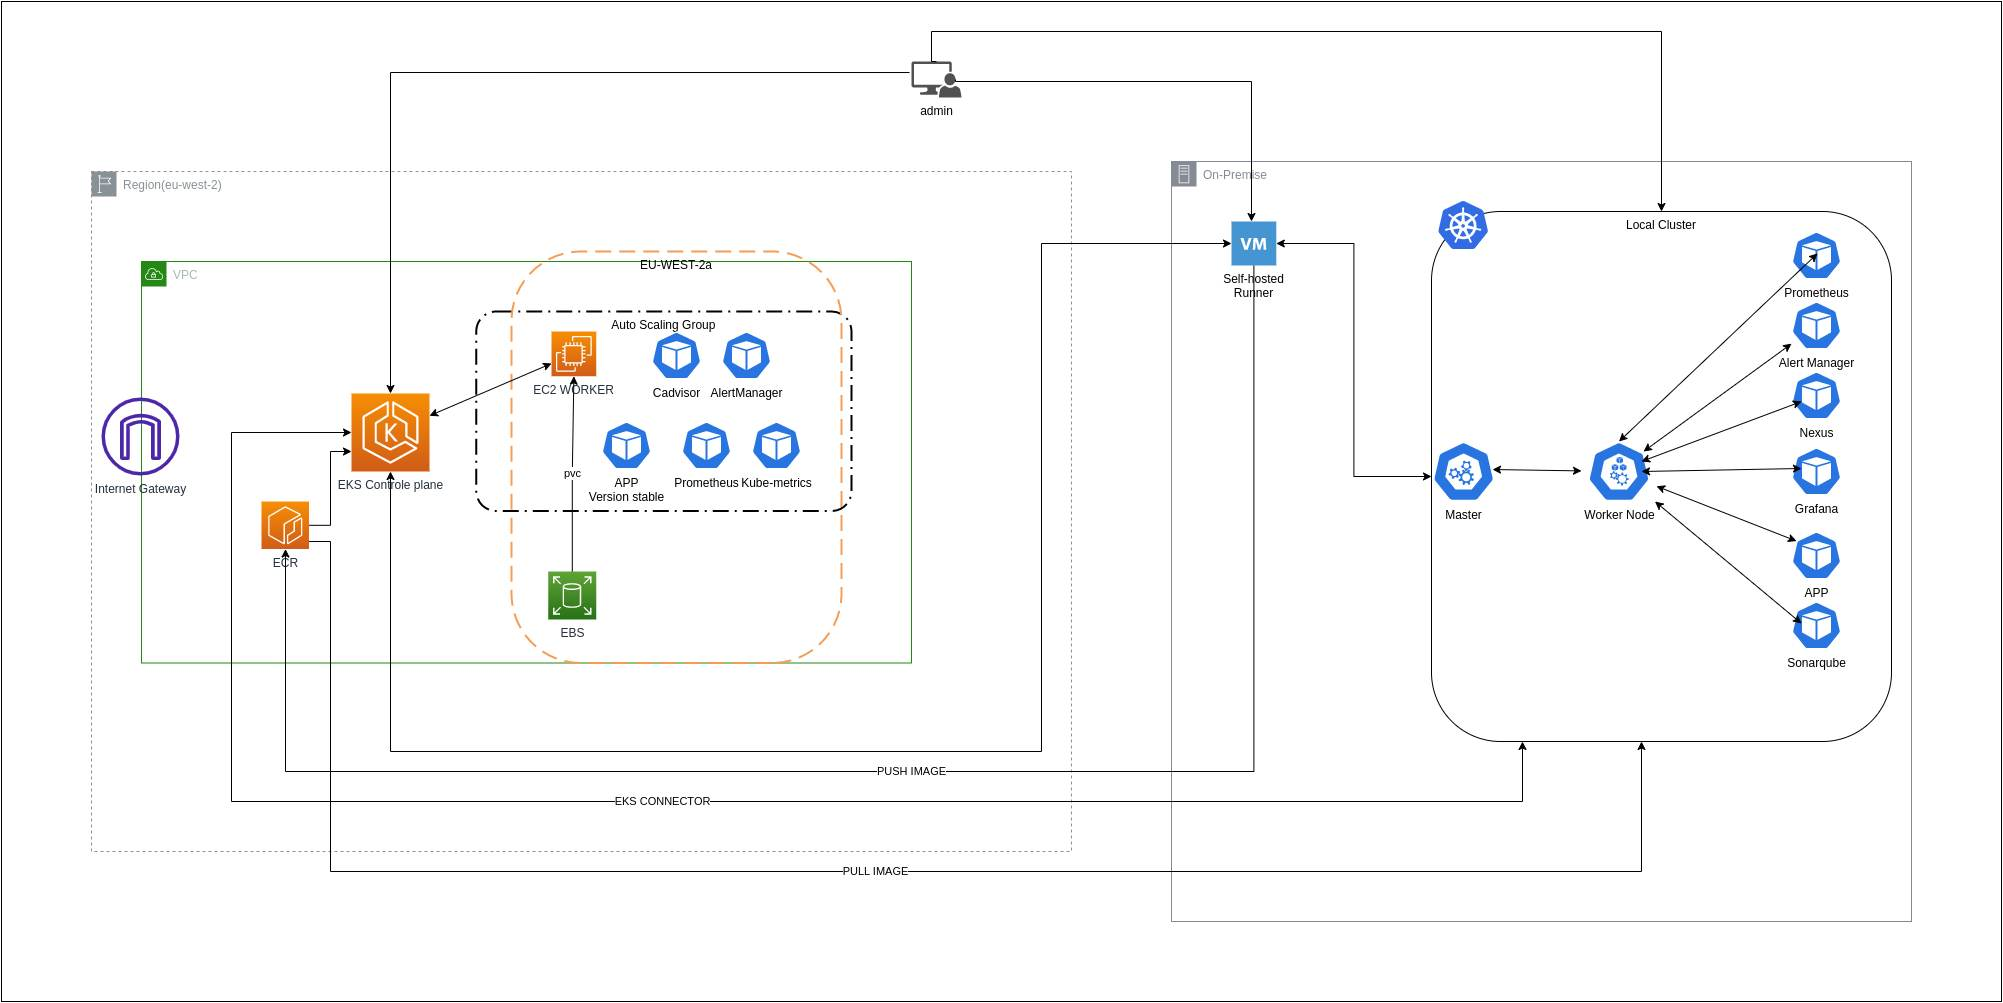
\includegraphics[height=16cm,width=19cm]{aws global architecture.drawio.png}
\end{center}
\caption{Architecture Cloud}
%\floatfoot{Source: (Citation command)}
% avec le package "floatrow"
\end{figure}

%footnote protected pour apparaitre dans la légende 

\section{\LARGE Architecture Détaillée}
\textsf{\fontfamily{qtm}\selectfont\scalefont{1.3}Dans cette partie nous allons présenter l'architecture détaillée correspond au sprint.}

\subsection{\Large Diagramme Cas d'utilisation Détaillée}
\textsf{\fontfamily{qtm}\selectfont\scalefont{1.3}Afin d'éliminer toute ambiguïté et de clarifier le cas d'utilisation, nous présentons le cas de façon détaillée.}
\begin{figure}[H]
    \begin{center}
    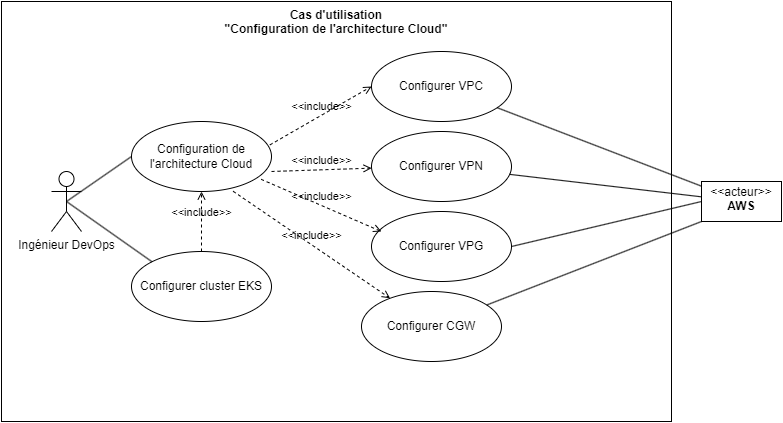
\includegraphics[height=10cm]{usecasedet.drawio.png}
    \end{center}
    \caption{cas d’utilisation"Configuration de l'architecture cloud AWS"}
    %\floatfoot{Source: (Citation command)}
    % avec le package "floatrow"
    \end{figure}
    \textsf{\fontfamily{qtm}\selectfont\scalefont{1.3}
    Pour expliquer  le diagramme de cas d’utilisation, nous représentons la description textuelle du principales fonctionnalités mentionnées ci-dessus : \\}
    \begin{center}
       \begin{table}[H]  
         \centering
         \resizebox{1.1\textwidth}{!}{%
         \begin{tabular}{|c|p{13cm}|}
          \hline
          Titre & Configuration de l'architecture cloud AWS\\
          \hline
          Acteur & Ingénieur DevOps \\
          \hline
          Description & L'ingénieur DevOps gérait la configuration de l'architecture et la création du cluster EKS.\\
          \hline
          Pré conditions & Connexion a amazon web services. \\
          \hline
          Post conditions & une architecture configurait correctement.  \\
          \hline 
          Scénario nominal & la connexion est réussite et la configuration réussite.\\
          \hline
          Scénario alternatif & La connexion échoue entre le cluster et la machine locale ou la configuration n'est pas correcte.  \\
          \hline
          \end{tabular}%
         }
       \caption{Description de cas d’utilisation}
       \end{table}
       \end{center}
\subsection{\Large Diagramme de séquence Détaillée}
\textsf{\fontfamily{qtm}\selectfont\scalefont{1.3}Nous détaillons ci-dessous les interactions générales du système }
\begin{figure}[H]
    \begin{center}
    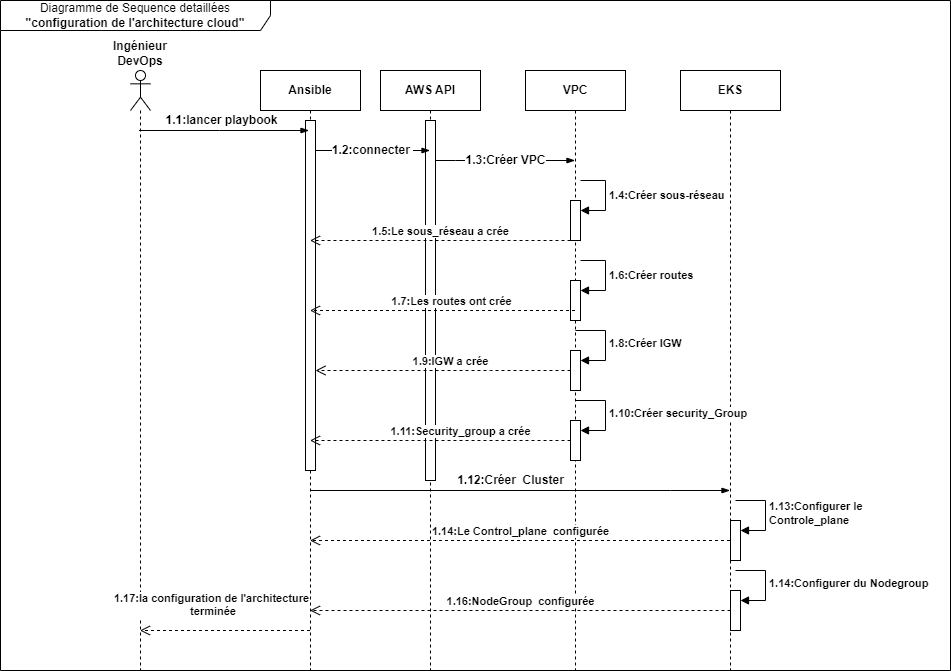
\includegraphics[height=15cm,width=18cm]{seqd.drawio.png}
    \end{center}
    \caption{Architecture Cloud}
    %\floatfoot{Source: (Citation command)}
    % avec le package "floatrow"
    \end{figure}




\section{Realisation}
% \begin{figure}[!ht]
%     \begin{center}
%     
\includegraphics[height=12cm]{autre_partie/image2}
%     \end{center}
%     \caption[autre partie]{autre partie globale de notre quelque chose}
%     \end{figure}

\section{Conclusion}
\newpage
\begin{figure}[H]
    \begin{center}
    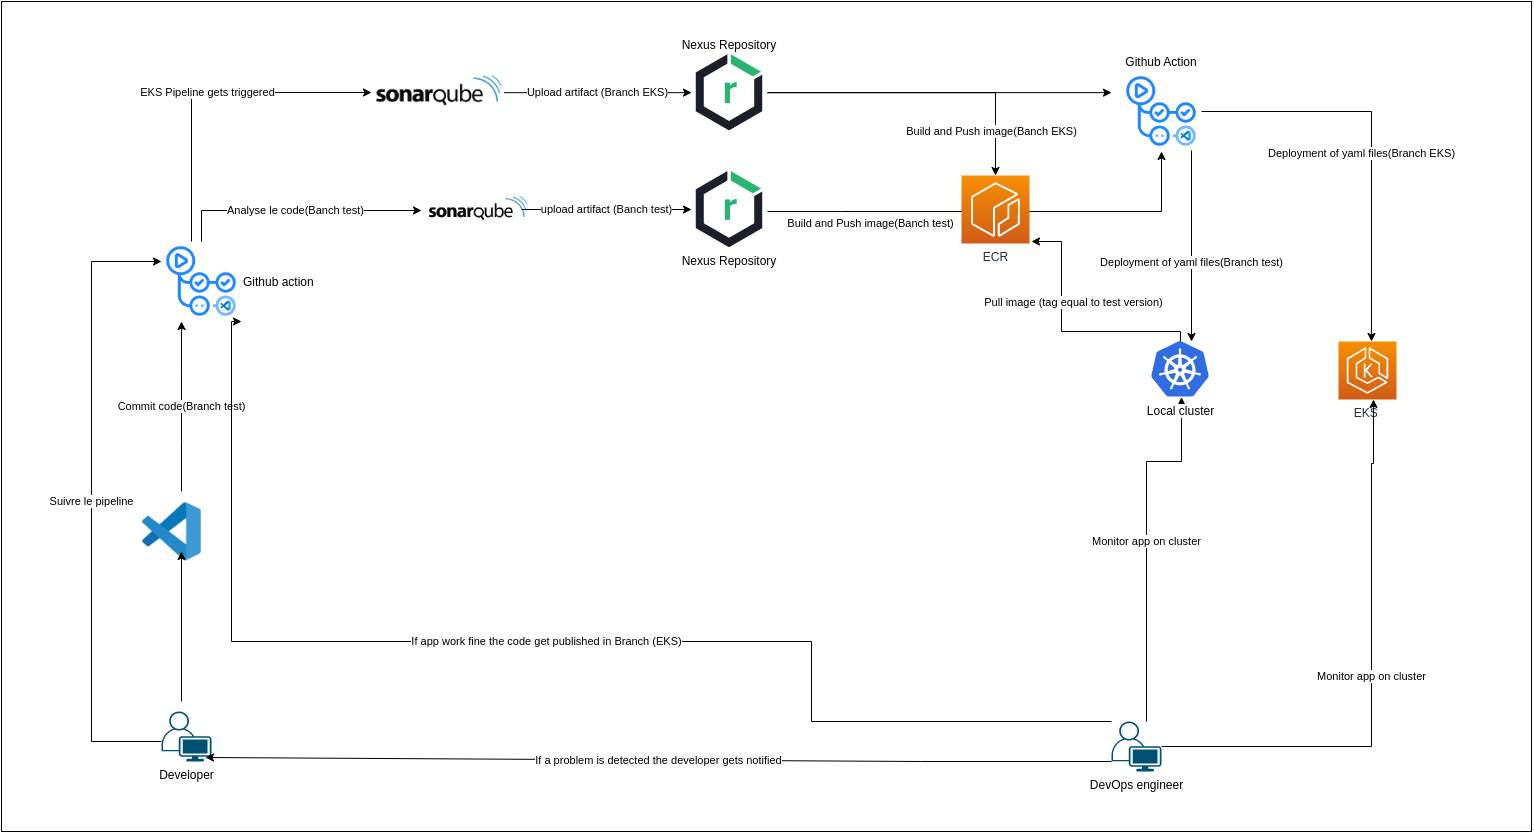
\includegraphics[height=17cm,width=18.5cm]{CI_CD EKS.drawio.png}
    \end{center}
    \caption{la configuration de pipeline}
    %\floatfoot{Source: (Citation command)}
    % avec le package "floatrow"
    \end{figure}
%Les lignes :
% \setcounter{secnumdepth}{4}
% \setcounter{tocdepth}{4}
%dans le fichier "main.tex" permettent de faire en sorte que les paragraphes soient interprété comme des titres de niveau 5
% \paragraph{Paragraphe 1 (agissant comme titre niveau 5)}
% %forcer un saut de ligne
% ~\\
% \hskip7mm

% \begin{figure}[!ht]
% \begin{center}
% 
\includegraphics[height=6cm]{autre_partie/image3}
% \end{center}
% \caption[Structure d'unz autre chose]{Structure d'une autre chose\protect\footnotemark}
% \end{figure}

% Ce schéma représente bla.

% \footnotetext{Schéma et explication d'après le wiki bla (cf. ref. \cite{cite0})}

% \paragraph{Paragraphe 2}
% ~\\
% \hskip7mm

% %fixer les floats précédemment définis
% %\FloatBarrier

% Bla

% \subparagraph{Sous-paragraphe 1}
% ~\\
% \hskip7mm

% Bla

% \begin{figure}[H]
% \begin{center}
% 
\includegraphics[height=10cm]{autre_partie/image4}
% \end{center}
% \caption{Diagramme de truc}
% \end{figure}

% \subparagraph{Sous-paragraphe 2}
% ~\\
% \hskip7mm

% Bla\\

% Bla

% \subparagraph{Sous-paragraphe 3}
% ~\\
% \hskip7mm

% Bla

% \subsubsection{Sous-sous-partie 3}

% Bla

% \section{Partie 2}

% Bla

% \footnotetext{D'après le schéma disponible sur la documentfation officielle disponible sur le site blalbla}

% Bla

% \subsection{Sous-partie 1}

% Bla

% \subsection{Sous-partie 2}

% Bla

% \paragraph*{Paragraphe 1 (n'apparaitra pas dans l'index)}
% Bla

% \paragraph*{Paragraphe 2}
% Bla

% \paragraph*{Paragraphe 3}
% Bla

% \subsection{Sous-partie 3}

% Bla